\documentclass[11pt,a4paper]{article}
\usepackage[utf8]{inputenc}
\usepackage[french]{babel}
\usepackage[T1]{fontenc}
\usepackage{amsmath}
\usepackage{amssymb}
\usepackage{graphicx}
\usepackage{geometry}
\usepackage{fancyhdr}
\usepackage{circuitikz}
\usepackage{pgfplots}
\usepackage{graphicx}
\usepackage{float}
\pgfplotsset{compat=1.18}

\geometry{margin=2cm}

% Configuration de l'en-tête
\pagestyle{fancy}
\fancyhf{} % Efface tous les en-têtes et pieds de page

% En-tête gauche
\fancyhead[L]{%
    \begin{tabular}[t]{@{}l@{}}
        \textbf{Nom:} KALIPE \\
        \textbf{Prénoms:} Kossi Mathias
    \end{tabular}%
}

% En-tête droite
\fancyhead[R]{%
    \begin{tabular}[t]{@{}l@{}}
        \textbf{}  \\
        \textbf{N° Étudiant:} 21507247
    \end{tabular}%
}

% Ligne horizontale sous l'en-tête
\renewcommand{\headrulewidth}{0.4pt}

% Pied de page (numéro de page centré)
\fancyfoot[C]{\thepage}

\title{\textbf{Préparation au TP\\Oscillateurs Sinusoïdaux}}
\author{Électronique des Systèmes Analogiques\\M1 SYSCOM | UM4EE101 - Sorbonne Université \\ \\ \textbf{N° Étudiant:} 21507247 \\ \textbf{Nom et prénoms:} KALIPE Kossi Mathias}

\date{}

\begin{document}

\maketitle

\section{Oscillateur à Pont de Wien}

\subsection{Conditions d'oscillations}

\subsubsection{Question 1 : Étude du réseau de réaction}

\begin{figure}[H]
    \centering
    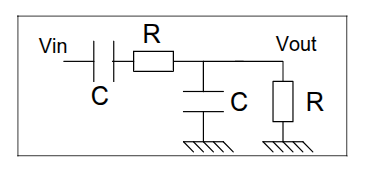
\includegraphics[width=0.5\linewidth]{images/reseau_reaction.png}
    \caption{Schéma du réseau de réaction}
    \label{fig:Schéma du réseau de réaction}
\end{figure}

\paragraph{Calcul de la fonction de transfert $\beta(j\omega)$}

Le réseau RC est constitué de deux branches :
\begin{itemize}
    \item Une branche série : $R$ et $C$ avec impédance $Z_1 = R + \frac{1}{j\omega C}$
    \item Une branche parallèle : $R$ et $C$ avec impédance $Z_2 = \frac{R \cdot \frac{1}{j\omega C}}{R + \frac{1}{j\omega C}}$
\end{itemize}

La fonction de transfert s'écrit :
\begin{equation}
\beta(j\omega) = \frac{V_{out}}{V_{in}} = \frac{Z_2}{Z_1 + Z_2}
\end{equation}

Avec $Z_2 = R \parallel \frac{1}{j\omega C}$, on a :
\begin{equation}
Z_2 = \frac{R}{1 + j\omega RC}
\end{equation}

Et :
\begin{equation}
Z_1 = R + \frac{1}{j\omega C} = \frac{Rj\omega C + 1}{j\omega C}
\end{equation}

Calculons $Z_1 + Z_2$ :
\begin{align}
Z_1 + Z_2 &= \frac{Rj\omega C + 1}{j\omega C} + \frac{R}{1 + j\omega RC} \\
&= \frac{(Rj\omega C + 1)(1 + j\omega RC) + Rj\omega C}{j\omega C(1 + j\omega RC)} \\
&= \frac{Rj\omega C + R^2j^2\omega^2C^2 + 1 + j\omega RC + Rj\omega C}{j\omega C(1 + j\omega RC)} \\
&= \frac{1 - \omega^2R^2C^2 + 3j\omega RC}{j\omega C(1 + j\omega RC)}
\end{align}

D'où :
\begin{equation}
\beta(j\omega) = \frac{Z_2}{Z_1 + Z_2} = \frac{\frac{R}{1 + j\omega RC}}{\frac{1 - \omega^2R^2C^2 + 3j\omega RC}{j\omega C(1 + j\omega RC)}}
\end{equation}

Simplifions :
\begin{equation}
\beta(j\omega) = \frac{Rj\omega C}{1 - \omega^2R^2C^2 + 3j\omega RC}
\end{equation}

En multipliant numérateur et dénominateur par $\frac{1}{j\omega RC}$ :
\begin{equation}
\beta(j\omega) = \frac{1}{3 + j\left(\frac{1}{\omega RC} - \omega RC\right)}
\end{equation}

En posant $\omega_0 = \dfrac{1}{RC}$ et $x = \dfrac{\omega}{\omega_0}$, on obtient :
\begin{equation}
\boxed{\beta(j\omega) = \frac{1}{3 + j\left(\frac{1}{x} - x\right)}}
\end{equation}

\textbf{Remarque :} À la fréquence $\omega_0$ ($x = 1$), la partie imaginaire s'annule, ce qui donne un déphasage nul.

\paragraph{Module et phase}

Le module de $\beta$ :
\begin{equation}
|\beta(j\omega)| = \frac{1}{\sqrt{9 + \left(\frac{1}{x} - x\right)^2}}
\end{equation}

À la fréquence $\omega_0$ (où $x=1$) :
\begin{equation}
\boxed{|\beta(j\omega_0)| = \frac{1}{3}}
\end{equation}

La phase :
\begin{equation}
\phi(\omega) = -\arctan\left(\frac{\frac{1}{x} - x}{3}\right)
\end{equation}

À $\omega_0$ : $\boxed{\phi(\omega_0) = 0°}$

\paragraph{Diagramme de Bode}

\begin{itemize}
    \item \textbf{Module} : Maximum de $-9.54$ dB à $\omega_0$, décroît de part et d'autre
    \item \textbf{Phase} : Passe de $+90°$ (BF) à $0°$ à $\omega_0$, puis à $-90°$ (HF)
\end{itemize}

\begin{figure}[H]
    \centering
    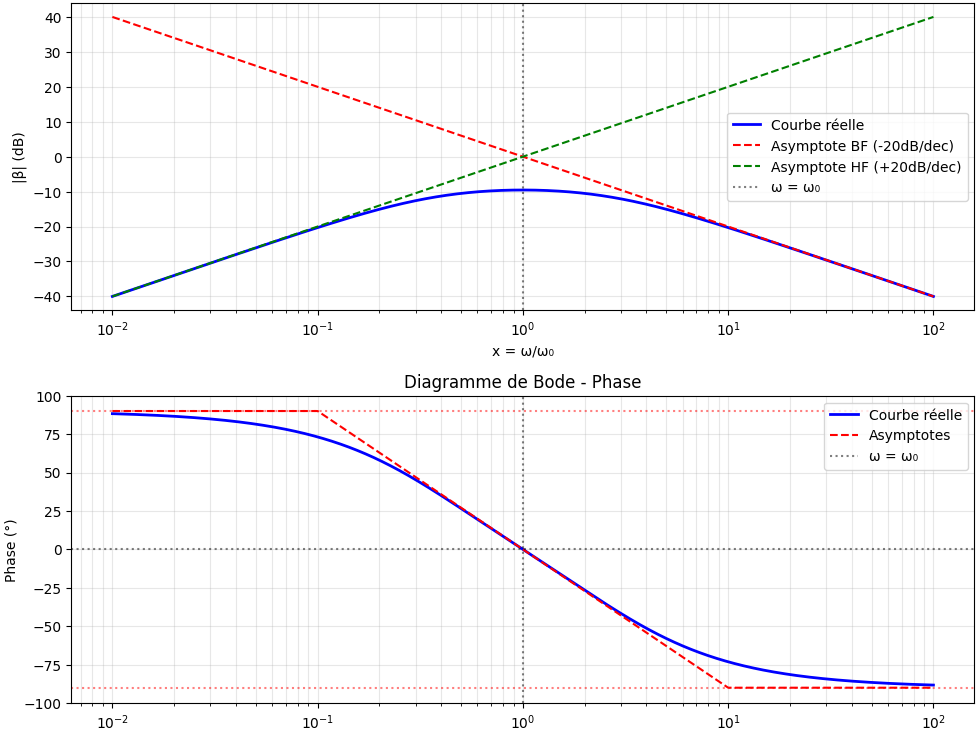
\includegraphics[width=0.8\linewidth]{images/bode_asympto_wien.png}
    \caption{Diagramme de Bode du réseau de réaction}
    \label{fig:Diagramme de Bode du réseau de réaction}
\end{figure}

\subsubsection{Question 2 : Conditions d'oscillations}

\paragraph{Données}
\begin{itemize}
    \item $R_1 = 1$ k$\Omega$
    \item $C = 2.2$ nF
    \item $f_{osc} = 10$ kHz
\end{itemize}

\paragraph{Fonction de transfert en boucle fermée}

L'amplificateur non-inverseur a un gain :
\begin{equation}
A = 1 + \frac{R_2}{R_1}
\end{equation}

La fonction de transfert en boucle ouverte :
\begin{equation}
T(j\omega) = A \cdot \beta(j\omega)
\end{equation}

\paragraph{Critère de Barkhausen}

Pour avoir des oscillations sinusoïdales, il faut :
\begin{equation}
\boxed{|T(j\omega_0)| = 1 \quad \text{et} \quad \arg(T(j\omega_0)) = 0° \text{ [2}\pi\text{]}}
\end{equation}

Puisque $|\beta(j\omega_0)| = \frac{1}{3}$ et $\arg(\beta(j\omega_0)) = 0°$ :

\begin{equation}
\boxed{A = 3 \quad \Rightarrow \quad 1 + \frac{R_2}{R_1} = 3 \quad \Rightarrow \quad R_2 = 2R_1}
\end{equation}

\paragraph{Calcul des valeurs}

Pour $f_{osc} = 10$ kHz :
\begin{equation}
\omega_0 = 2\pi f_{osc} = \frac{1}{RC}
\end{equation}

D'où :
\begin{equation}
R = \frac{1}{2\pi f_{osc} \cdot C} = \frac{1}{2\pi \times 10^4 \times 2.2 \times 10^{-9}}
\end{equation}

\begin{equation}
\boxed{R = 7234 \, \Omega \approx 7.2 \, \text{k}\Omega}
\end{equation}

Et avec $R_1 = 1$ k$\Omega$ :
\begin{equation}
\boxed{R_2 = 2 \, \text{k}\Omega}
\end{equation}

\paragraph{Comportement selon |T|}

\begin{itemize}
    \item \textbf{Si $|T| < 1$} : Les oscillations s'amortissent exponentiellement et disparaissent progressivement
    \item \textbf{Si $|T| > 1$} : Les oscillations croissent exponentiellement jusqu'à saturation aux tensions d'alimentation, créant une distorsion harmonique importante
    \item \textbf{Si $|T| = 1$} : Oscillations sinusoïdales entretenues d'amplitude constante (condition théorique idéale)
\end{itemize}

\subsection{Stabilisation de l'amplitude des oscillations}

\subsubsection{Question 1 : Résistance commandée en tension}

\paragraph{Choix de la résistance à remplacer}

Il faut remplacer \textbf{$R_2$} par la résistance commandée en tension $(R' + R_{DS})$.

\paragraph{Justification}

Le gain de l'amplificateur est :
\begin{equation}
A = 1 + \frac{R_2}{R_1}
\end{equation}

Pour stabiliser l'amplitude par contre-réaction négative :
\begin{itemize}
    \item Si l'amplitude \textbf{augmente} : on veut \textbf{diminuer le gain} $\Rightarrow$ diminuer $R_2$
    \item Si l'amplitude \textbf{diminue} : on veut \textbf{augmenter le gain} $\Rightarrow$ augmenter $R_2$
\end{itemize}

Avec le FET (canal N à déplétion) en série avec $R'$ pour former $R_2$ :
\begin{itemize}
    \item Amplitude trop forte $\Rightarrow$ $|V_g|$ augmente (plus négatif) $\Rightarrow$ $R_{DS}$ augmente $\Rightarrow$ gain diminue
    \item Amplitude trop faible $\Rightarrow$ $|V_g|$ diminue (moins négatif) $\Rightarrow$ $R_{DS}$ diminue $\Rightarrow$ gain augmente
\end{itemize}

C'est donc une \textbf{contre-réaction automatique} qui stabilise l'amplitude autour de la valeur de consigne.

\subsubsection{Question 2 : Génération de la tension de commande}

\begin{figure}[H]
    \centering
    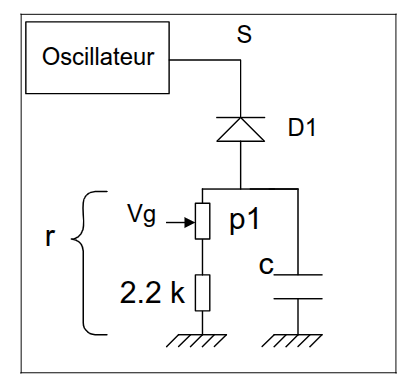
\includegraphics[width=0.8\linewidth]{images/tension_commande.png}
    \caption{Circuit de génération de la tension de commande $V_g$}
    \label{fig:Circuit de commande}
\end{figure}

\paragraph{Fonctionnement du circuit}

Le montage comprend :
\begin{itemize}
    \item \textbf{Diode $D_1$} : Redressement mono-alternance (détection des crêtes positives)
    \item \textbf{Filtre RC ($r$, $c$)} : Lissage pour obtenir une tension continue proportionnelle à l'amplitude crête
    \item \textbf{Potentiomètre $p_1$ (10 k$\Omega$)} : Diviseur de tension ajustable pour fixer le point de fonctionnement du FET
    \item \textbf{Résistance de 2.2 k$\Omega$} : Partie inférieure du diviseur résistif
\end{itemize}

\paragraph{Choix de la constante $\tau = rc$}

La constante de temps doit être suffisamment grande pour filtrer efficacement la composante alternative à $f_{osc}$ :
\begin{equation}
\tau \gg T_{osc} = \frac{1}{f_{osc}}
\end{equation}

Pour $f_{osc} = 10$ kHz : $T_{osc} = 100$ µs

On choisit : $\tau \approx (50 \text{ à } 100) \times T_{osc}$ pour un bon filtrage

Avec $r = 2.2$ k$\Omega$ et $\tau = 100 \times 100 \times 10^{-6} = 10$ ms :
\begin{equation}
c = \frac{\tau}{r} = \frac{10 \times 10^{-3}}{2200} = 4.54 \times 10^{-6} \text{ F}
\end{equation}

\begin{equation}
\boxed{c \approx 4.7 \, \mu\text{F}}
\end{equation}

\paragraph{Réglage de $p_1$ pour $V_g = -2$ V}

L'amplitude crête de sortie souhaitée est $V_{crête} = 8$ V.

Après redressement et filtrage, la tension continue aux bornes de $c$ vaut approximativement :
\begin{equation}
V_c \approx V_{crête} - V_D \approx 8 - 0.6 = 7.4 \text{ V}
\end{equation}

Cette tension est appliquée au diviseur résistif formé par le potentiomètre $p_1$ (10 k$\Omega$) et la résistance de 2.2 k$\Omega$ vers la masse.

Pour obtenir $V_g = -2$ V à la grille, il faut positionner le curseur de $p_1$ de façon à ce que :
\begin{equation}
V_g = -V_c \times \frac{2.2}{x + 2.2}
\end{equation}

où $x$ est la partie du potentiomètre entre le curseur et la tension $V_c$.

Pour $|V_g| = 2$ V :
\begin{equation}
2 = 7.4 \times \frac{2.2}{x + 2.2}
\end{equation}

\begin{equation}
x + 2.2 = 7.4 \times \frac{2.2}{2} = 8.14
\end{equation}

\begin{equation}
x = 8.14 - 2.2 = 5.94 \text{ k}\Omega
\end{equation}

\textbf{Position du curseur :} Le curseur doit être positionné à environ \boxed{60\%} de la course du potentiomètre (depuis le point connecté à $V_c$).

\paragraph{Valeur de $R'$}

D'après le tableau, pour $V_{GS} = -2$ V : $R_{DS} = 230$ $\Omega$

Le gain nécessaire est $A = 3$, donc :
\begin{equation}
R_2 = R' + R_{DS} = 2 \times R_1 = 2000 \, \Omega
\end{equation}

\begin{equation}
\boxed{R' = 2000 - 230 = 1770 \, \Omega \approx 1.8 \, \text{k}\Omega}
\end{equation}

\subsection{Influence des performances de l'amplificateur opérationnel}

\subsubsection{Question 1 : Bande passante en petits signaux}

\paragraph{Données}
\begin{itemize}
    \item TL081 : GBW = 3 MHz
    \item A741 : GBW = 1 MHz
    \item Gain du montage : $A = 3$
\end{itemize}

\paragraph{Calcul de la bande passante}

Pour un amplificateur opérationnel avec compensation interne, la bande passante en boucle fermée est donnée par :
\begin{equation}
BP = \frac{GBW}{A}
\end{equation}

Pour le TL081 :
\begin{equation}
\boxed{BP_{TL081} = \frac{3 \times 10^6}{3} = 1 \, \text{MHz}}
\end{equation}

Pour le A741 :
\begin{equation}
\boxed{BP_{A741} = \frac{1 \times 10^6}{3} = 333 \, \text{kHz}}
\end{equation}

\paragraph{Effet à 10 kHz}

La fréquence d'oscillation (10 kHz) est \textbf{très inférieure} aux bandes passantes calculées :
\begin{itemize}
    \item $f_{osc} / BP_{TL081} = 10/1000 = 1\%$
    \item $f_{osc} / BP_{A741} = 10/333 = 3\%$
\end{itemize}

$\Rightarrow$ \textbf{Aucun effet sensible} en petits signaux. Les deux amplificateurs opérationnels présentent un gain pratiquement constant et un déphasage négligeable à 10 kHz. Les conditions d'oscillations sont respectées avec les deux composants.

\subsubsection{Question 2 : Fonctionnement en grands signaux}

\paragraph{Vitesse de balayage nécessaire}

Pour une sinusoïde $v(t) = V_{crête} \sin(\omega t)$ avec $V_{crête} = 8$ V et $f = 10$ kHz :

\begin{equation}
\frac{dv}{dt} = V_{crête} \omega \cos(\omega t)
\end{equation}

La pente maximale (vitesse de balayage nécessaire) est :
\begin{equation}
\left|\frac{dv}{dt}\right|_{max} = V_{crête} \times 2\pi f = 8 \times 2\pi \times 10^4 = 502.7 \times 10^3 \text{ V/s}
\end{equation}

\begin{equation}
\boxed{SR_{nécessaire} = 0.50 \, \text{V}/\mu\text{s}}
\end{equation}

\paragraph{Comparaison avec les Slew Rates}

\begin{itemize}
    \item TL081 : SR = 13 V/µs $\gg$ 0.50 V/µs $\Rightarrow$ \textbf{Aucune limitation, signal parfait}
    \item A741 : SR = 0.5 V/µs $\approx$ 0.50 V/µs $\Rightarrow$ \textbf{Limitation critique}
\end{itemize}

\paragraph{Formes d'onde attendues}

\begin{itemize}
    \item \textbf{TL081} : Signal sinusoïdal pur à 10 kHz, sans distorsion
    \item \textbf{A741} : Signal sinusoïdal avec légère distorsion sur les fronts montants et descendants. La vitesse de variation étant limitée à 0.5 V/µs, les zones de forte pente sont légèrement « écrêtées », donnant un aspect légèrement triangulaire. La fréquence reste à 10 kHz.
\end{itemize}

\subsubsection{Question 3 : Avec $C = 1$ nF}

\paragraph{Nouvelle fréquence d'oscillation}

La fréquence d'oscillation est inversement proportionnelle à $C$ :
\begin{equation}
f_{osc} = \frac{1}{2\pi RC}
\end{equation}

Si $C$ passe de 2.2 nF à 1 nF (divisée par 2.2) :
\begin{equation}
f_{nouvelle} = f_{ancienne} \times \frac{2.2}{1} = 10 \times 2.2 = 22 \, \text{kHz}
\end{equation}

\paragraph{Bande passante (Reprise de III.1)}

Les bandes passantes restent identiques (elles ne dépendent que du GBW et du gain) :
\begin{itemize}
    \item TL081 : 1 MHz $\gg$ 22 kHz $\Rightarrow$ Toujours OK
    \item A741 : 333 kHz $\gg$ 22 kHz $\Rightarrow$ Toujours OK
\end{itemize}

\textbf{Conclusion :} En petits signaux, aucun problème avec les deux composants à 22 kHz.

\paragraph{Slew Rate (Reprise de III.2)}

La vitesse de balayage nécessaire à 22 kHz :
\begin{equation}
SR_{nécessaire} = 8 \times 2\pi \times 22 \times 10^3 = 1.106 \times 10^6 \text{ V/s}
\end{equation}

\begin{equation}
\boxed{SR_{nécessaire} = 1.11 \, \text{V}/\mu\text{s}}
\end{equation}

\textbf{Comparaison :}
\begin{itemize}
    \item TL081 : 13 V/µs $\gg$ 1.11 V/µs $\Rightarrow$ \textbf{Signal sinusoïdal parfait}
    \item A741 : 0.5 V/µs $<$ 1.11 V/µs $\Rightarrow$ \textbf{Forte distorsion}
\end{itemize}

\textbf{Avec le A741 à 22 kHz :} Le signal de sortie présente une forte limitation de vitesse. Le SR disponible étant inférieur de plus de 50\% au SR nécessaire, le signal prend une forme \textbf{triangulaire} prononcée. 

\boxed{\text{Le A741 est inadapté à 22 kHz pour des signaux de 8 V d'amplitude}}

\section{Oscillateur à Déphasage}

\subsection{Question 1 : Étude du réseau RC}

\begin{figure}[H]
    \centering
    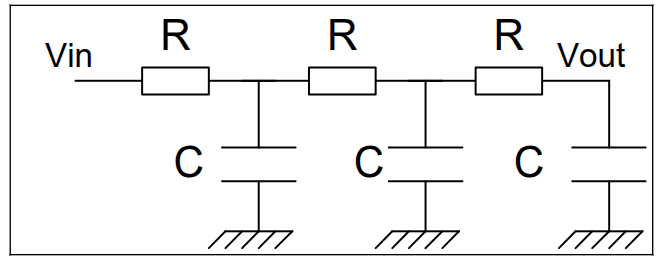
\includegraphics[width=0.5\linewidth]{images/rc_dephasage.png}
    \caption{Schéma du réseau déphasant}
    \label{fig:Schéma du réseau déphasant}
\end{figure}

\paragraph{Plage de variation de la phase}

Ce réseau est constitué de 3 cellules RC passe-bas identiques en cascade.

Chaque cellule RC passe-bas introduit un déphasage compris entre 0° et -90° :
\begin{itemize}
    \item À \textbf{basse fréquence} ($\omega \to 0$) : Les capacités se comportent comme des circuits ouverts $\Rightarrow$ aucun déphasage $\Rightarrow$ $\phi_{cellule} = 0°$
    \item À \textbf{haute fréquence} ($\omega \to \infty$) : Les capacités se comportent comme des court-circuits $\Rightarrow$ déphasage maximal $\Rightarrow$ $\phi_{cellule} = -90°$
\end{itemize}

Pour 3 cellules en cascade :
\begin{equation}
\boxed{\phi_{total} \in [0°, -270°]}
\end{equation}

\paragraph{Utilisation avec amplificateur inverseur}

Un amplificateur \textbf{inverseur} introduit un déphasage de $-180°$ (ou $+180°$, équivalent).

Pour satisfaire le critère d'oscillation de Barkhausen, la phase totale en boucle ouverte doit être un multiple de $360°$ :
\begin{equation}
\phi_{total} = \phi_{ampli} + \phi_{RC} = n \times 360°
\end{equation}

Avec un amplificateur inverseur :
\begin{equation}
-180° + \phi_{RC} = 0° \quad \Rightarrow \quad \phi_{RC} = +180° = -180° \text{ [360°]}
\end{equation}

Comme le réseau RC peut fournir une phase comprise entre 0° et -270°, il **peut** produire un déphasage de -180°.

$\Rightarrow$ \boxed{\text{COMPATIBLE avec un amplificateur inverseur}}

\paragraph{Avec amplificateur non-inverseur}

Un amplificateur \textbf{non-inverseur} n'introduit aucun déphasage ($\phi_{ampli} = 0°$).

Pour avoir des oscillations :
\begin{equation}
0° + \phi_{RC} = 0° \text{ [360°]} \quad \Rightarrow \quad \phi_{RC} = 0° \text{ ou } -360°
\end{equation}

Or, le réseau RC ne peut fournir qu'un déphasage compris entre 0° et -270°. Il ne peut donc pas atteindre -360°.

À $\phi_{RC} = 0°$ (basse fréquence), l'atténuation du réseau est très faible (proche de 1), ce qui ne permet pas de satisfaire simultanément la condition d'amplitude ($|T| = 1$) avec un gain d'amplificateur raisonnable.

$\Rightarrow$ \boxed{\text{NON COMPATIBLE en pratique avec un amplificateur non-inverseur}}

\paragraph{Mesure à l'oscilloscope pour déterminer les paramètres d'oscillation}

Pour caractériser expérimentalement le réseau RC :

\begin{enumerate}
    \item Alimenter $V_{in}$ avec un générateur basse fréquence (GBF) délivrant un signal sinusoïdal d'amplitude constante
    \item Connecter la voie 1 de l'oscilloscope à $V_{in}$ et la voie 2 à $V_{out}$
    \item Balayer la fréquence du GBF (par exemple de 1 kHz à 100 kHz)
    \item Mesurer simultanément l'amplitude et le déphasage entre $V_{in}$ et $V_{out}$
    \item Identifier la fréquence $f_0$ où le déphasage vaut $\phi = -180°$ (les deux signaux sont en opposition de phase)
    \item À cette fréquence, mesurer le rapport d'amplitudes $|\beta| = \frac{V_{out}}{V_{in}}$
    \item Le gain de l'amplificateur inverseur devra être $|A| = \frac{1}{|\beta|}$ pour satisfaire le critère de Barkhausen
\end{enumerate}

\paragraph{Calcul de la fonction de transfert}

Pour calculer la fonction de transfert du réseau, on applique successivement les diviseurs de tension.

Soit $V_1$, $V_2$ et $V_3 = V_{out}$ les tensions aux nœuds intermédiaires.

En utilisant l'analyse nodale et après développements algébriques, on obtient :

\begin{equation}
\boxed{\beta(j\omega) = \frac{1}{1 - 5(\omega RC)^2 + j\omega RC[6 - (\omega RC)^2]}}
\end{equation}

\paragraph{Fréquence d'oscillation}

Pour un oscillateur avec amplificateur inverseur, le critère de phase impose :
\begin{equation}
\arg[\beta(j\omega)] = -180°
\end{equation}

Ceci correspond à une partie imaginaire négative avec un dénominateur réel négatif, ou une partie imaginaire nulle avec un numérateur et un dénominateur de signes opposés.

La partie imaginaire du dénominateur est :
\begin{equation}
\text{Im}[dénominateur] = \omega RC[6 - (\omega RC)^2]
\end{equation}

Pour $\phi = \pm 180°$, il faut que la partie réelle soit négative et la partie imaginaire nulle :
\begin{equation}
6 - (\omega RC)^2 = 0 \quad \Rightarrow \quad \omega^2R^2C^2 = 6
\end{equation}

Vérifions que la partie réelle est bien négative :
\begin{equation}
\text{Re}[dénominateur] = 1 - 5 \times 6 = 1 - 30 = -29 < 0
\end{equation}

Le numérateur étant réel positif (égal à 1), $\beta$ est bien réel négatif, donc $\arg[\beta] = -180°$.


D'où :
\begin{equation}
\boxed{\omega_{osc} = \frac{\sqrt{6}}{RC} \quad \Rightarrow \quad f_{osc} = \frac{\sqrt{6}}{2\pi RC}}
\end{equation}

\subsection{Question 2 : Dimensionnement de l'oscillateur}

\begin{figure}[H]
    \centering
    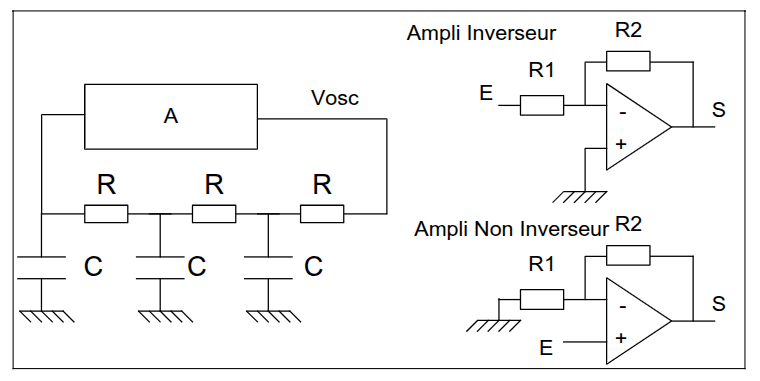
\includegraphics[width=0.8\linewidth]{images/oscillation_dephasage_rc.png}
    \caption{Dimensionnement de l'oscillateur}
    \label{fig:Dimensionnement de l'oscillateur}
\end{figure}

\paragraph{Gain nécessaire de l'amplificateur}
À la fréquence d'oscillation $f_{osc}$, on a $\omega_{osc}^2R^2C^2 = 6$.
Injectons cela dans la partie réelle du dénominateur de $\beta$ :
\begin{equation}
|\beta(j\omega_{osc})| = \frac{1}{|(1 - 5\omega_{osc}^2R^2C^2) + j \cdot 0|} = \frac{1}{|1 - 5 \times 6|}
\end{equation}
\begin{equation}
|\beta(j\omega_{osc})| = \frac{1}{|1 - 30|} = \frac{1}{29}
\end{equation}
Pour le critère de Barkhausen, $|A \cdot \beta| = 1$, donc le gain de l'ampli doit compenser cette atténuation :
\begin{equation}
\boxed{A = \frac{1}{|\beta|} = 29}
\end{equation}

\paragraph{Calcul de R et R2 pour $f_{osc} = 20$ kHz}
Données : $C = 10$ nF, $R_1 = 10$ k$\Omega$, $f_{osc} = 20$ kHz

De $f_{osc} = \frac{\sqrt{6}}{2\pi RC}$ :
\begin{equation}
R = \frac{\sqrt{6}}{2\pi f_{osc} C} = \frac{\sqrt{6}}{2\pi \times 20 \times 10^3 \times 10 \times 10^{-9}}
\end{equation}
\begin{equation}
\boxed{R = 1949 \, \Omega \approx 2 \, \text{k}\Omega}
\end{equation}

Pour le gain :
\begin{itemize}
    \item \textbf{Amplificateur inverseur} : $A = -\frac{R_2}{R_1} = -29$ $\Rightarrow$ $\boxed{R_2 = 290 \, \text{k}\Omega}$
    \item \textbf{Amplificateur non-inverseur} : $A = 1 + \frac{R_2}{R_1} = 29$ $\Rightarrow$ $\boxed{R_2 = 280 \, \text{k}\Omega}$
\end{itemize}

\paragraph{Avec $C = 1$ nF et $R \times 10$}

Si $C$ est divisé par 10 et $R$ multiplié par 10, le produit $RC$ reste constant.

D'après $f_{osc} = \frac{\sqrt{6}}{2\pi RC}$ :

\begin{equation}
\boxed{\text{OUI, le montage oscille à la même fréquence (20 kHz)}}
\end{equation}

\textbf{Justification} : La fréquence d'oscillation ne dépend que du produit $RC$, qui est conservé.

\vspace{1cm}

\end{document}